\begin{theo}[Wrijvingskracht]{Wrijvingskracht}

    De wrijvingkracht is de weerstand die het voorwerp ondervindt wanneer het over het oppervlak van een ander voorwerp beweegt. We bespreken 2 soorten wrijvingskrachten:
    
    \begin{itemize}
        \item \textbf{Kinetische:} $ F_k = \mu_kF_N$ met $ \mu_k $ de \textbf{kinetische} wrijvingscoëffiënt. Deze kracht is recht evenredig met de normaalkracht.
        \item \textbf{Statische:} $ F_s \leq \mu_sF_N$ met $ \mu_s $ de \textbf{statische} wrijvingscoëffiënt. Als deze drempelwaarde bereikt is, dan zal het object beginnen met bewegen en zal er sprake zijn van kinetische wrijving.
    \end{itemize}
    
    \noindent Er geldt dat het moeilijker is om een voorwerp te laten starten dan om een beweging verder te laten verlopen, of in formule vorm: 
    
    \vspace{-0.2cm}
    \begin{equation*}
        \mu_s > \mu_k
    \end{equation*} 
    \vspace{-0.4cm}
\end{theo}

% \begin{ex}[Voorbeeld: Wrijvingskracht]{Voorbeeld: Wrijvingskracht1}
%         \centering
%         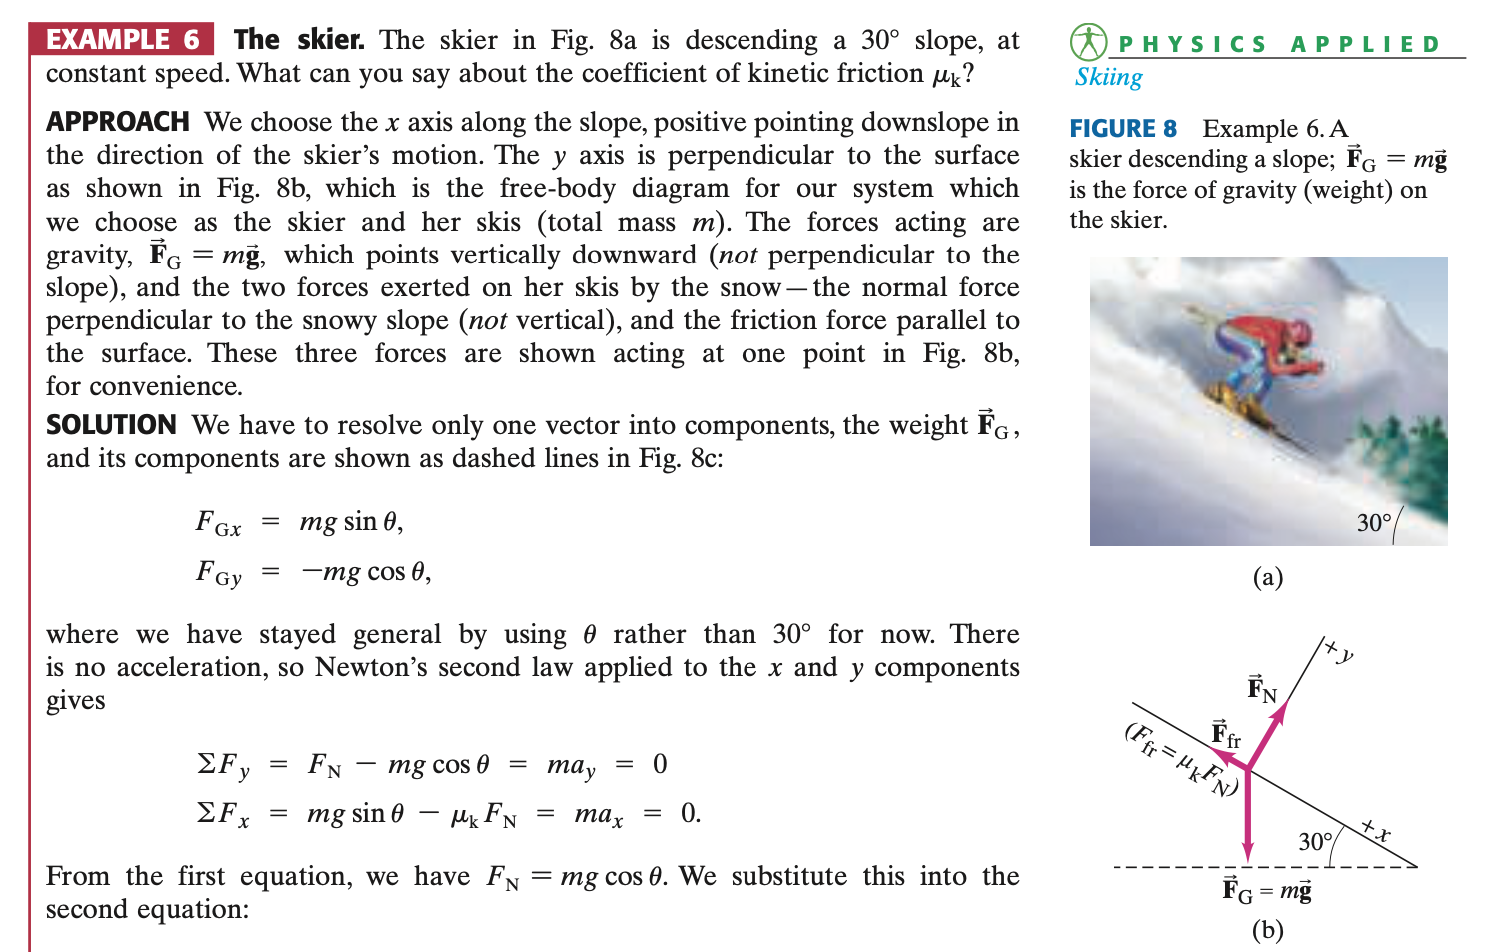
\includegraphics[scale = 0.6]{Examples/Dynamica/5.6.1.png}
%         \centering
%         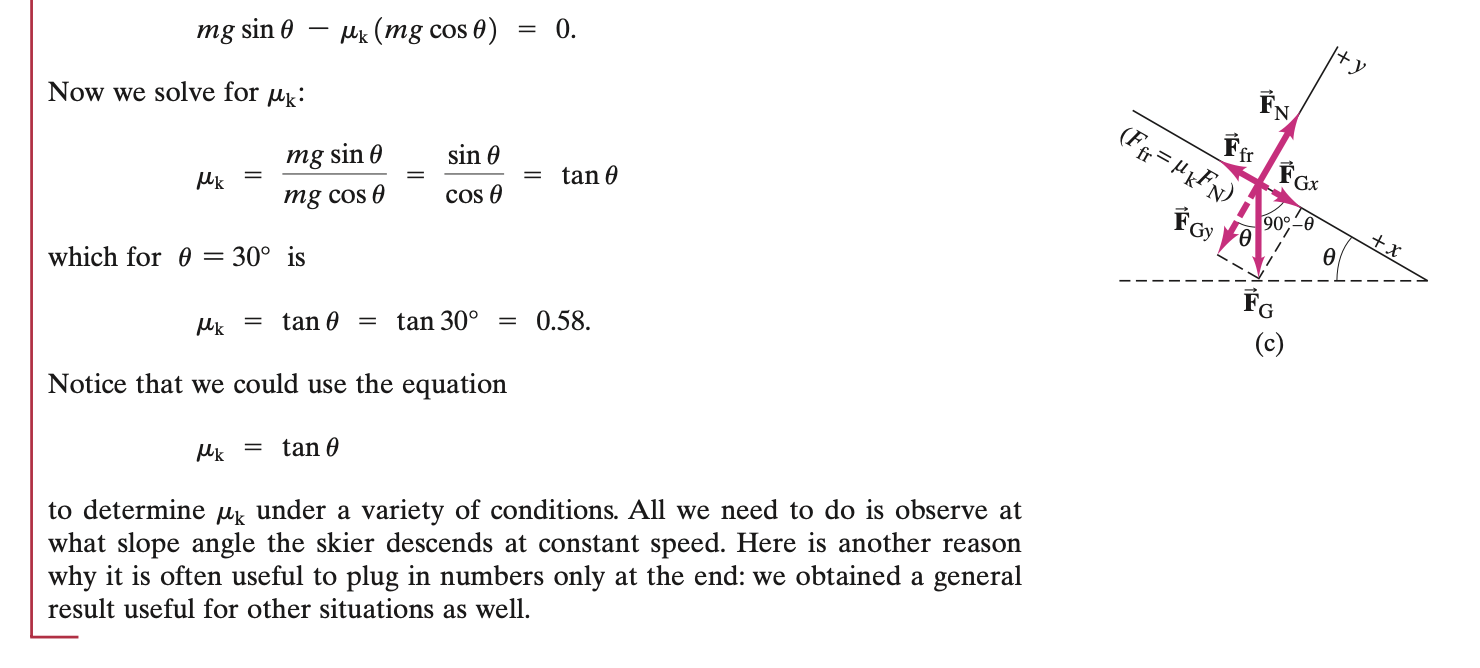
\includegraphics[scale = 0.6]{Examples/Dynamica/5.6.2.png}
%         \vspace{-0.5cm}
% \end{ex}

\begin{theo}[Kinematica van de eenparige cirkelbeweging]{Kinematica van de eenparige cirkelbeweging}
    \vspace{-0.4cm}
    \begin{minipage}{.71\textwidth}
        % We berekenen de versnelling door te vertrekken van de formule:
        % \begin{equation}
        %     \Vec{a} = \lim_{\Delta t \to 0} \dfrac{\Delta \Vec{v}}{\Delta t} = \dfrac{d\Vec{v}}{dt}
        % \end{equation}
        Een voorwerp dat met een constante snelheid in een cirkel beweegt voert een \textbf{eenparig cirkelvormige beweging} uit. In dit soort beweging blijft de grootte van de snelheidsvector constant, maar verandert de richting continu, m.a.w. $ a \neq 0 $. Uit gelijkvormige driehoeken volgt: 
    
        \begin{equation*}
            \dfrac{\Delta v}{v} \approx \dfrac{\Delta \ell}{r} \to \Delta v \approx \dfrac{v}{r}\Delta \ell
        \end{equation*}

        % \begin{center}
        %     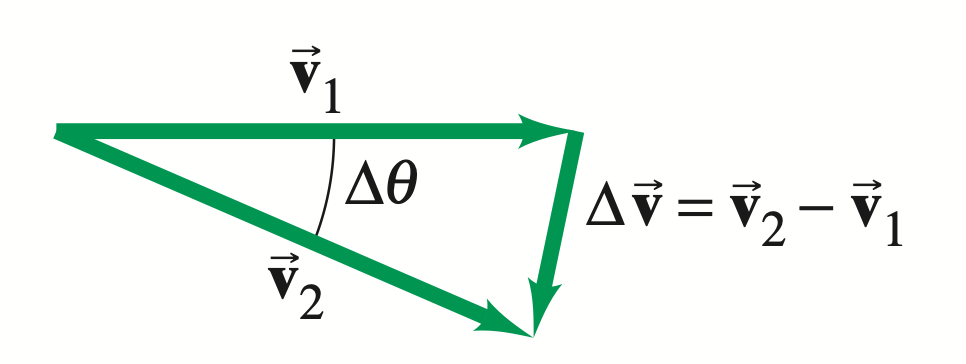
\includegraphics[scale = 0.25]{Images/Dynamica/Gelijkvormige driehoeken stap.png}
        % \end{center}
        
        \noindent en hiermuit kunnen we de middelpuntzoekende versnelling berekenen
        \begin{equation*}
            a_R = \lim_{\Delta t \to 0} \frac{\Delta v}{\Delta t} = \lim_{\Delta t \to 0} \frac{v}{r}\frac{\Delta \ell}{\Delta t} = \frac{v^2}{r}
        \end{equation*}
    \end{minipage} 
    \begin{minipage}{.25\textwidth}
        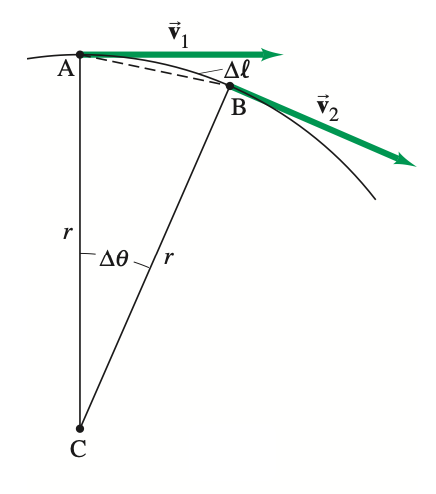
\includegraphics[scale = 0.3]{Images/Dynamica/Kinematica van de Cirkelbeweging.png}      
    \end{minipage}
    \vspace{0.3cm}

    \noindent Deze versnelling wordt de \textbf{centripetale versnelling} genoemd en is gericht naar het middelpunt van de cirkel. De snelheid van een ECB wordt gegeven door de volgende formule: 
    \begin{equation*}
        v = \dfrac{2\pi r}{T}
    \end{equation*}
    \noindent Hierbij is T de periode, m.a.w. tijd nodig voor een complete omwenteling. De frequentie van de ECB, m.a.w het aantal omwentelingen per seconde, wordt gegeven door de volgende formule
    \begin{equation*}
        f = \dfrac{1}{T} = \dfrac{v}{2\pi r} = \dfrac{\omega}{2\pi}
    \end{equation*}
    waarbij de dimensie Hz is.
\end{theo}

\newpage

\begin{theo}[Dynamica van de eenparige cirkelbeweging]{Dyamica van de eenparige cirkelbeweging}
    De cirkelbeweging is een versnelde beweging, dus er is een resulterende kracht nodig om het voorwerp op de cirkelbaan te houden, namelijk de \textbf{centripetale kracht}:

    \begin{equation*}
        (\sum F)_R = ma_R = m\dfrac{v^2}{r}
    \end{equation*}
    
    \noindent Om een voorwerp op een cirkelbaan te houden is er een centripetale versnelling en zoals hierboven vermeld een centripetale kracht nodig, dus de $ F_{net} $ moet naar het midden van de cirkel gericht zijn. Als deze kracht er niet is, dan zal het volgens de \textbf{Inertiewet} rechtlijnig zich voortbewegen.
\end{theo}
 
\begin{theo}[Kinematica én Dynamica niet-eenparige cirkelbeweging]{Niet-eenparige cirkelbeweging}
    In dit soort beweging beweegt het voorwerp volgens een cirkelbaan, maar kan het versnellen. De totale vectoriele versnelling in dit soort beweging wordt gegeven door de volgende formule:
    \begin{equation*}
        \Vec{a} = \Vec{a}_{tan} + \Vec{a}_R 
    \end{equation*}

    \noindent Sinds $ \Vec{a}_R $ en $ \Vec{a}_{tan} $ altijd loodrecht op elkaar staan, geldt op eenderwelk ogenblik:
        \begin{equation*}
            a = \sqrt{a_{tan}^2 + a_R^2} \text{ met } a_R = \dfrac{v^2}{r} \text{ en } a_{tan} = \dfrac{dv}{dt}
        \end{equation*}

    \noindent De figuren tonen de tangentiele en centripetale krachten en versnellingen bij een niet-eenparige cirkelbeweging:
    
        \begin{center}
            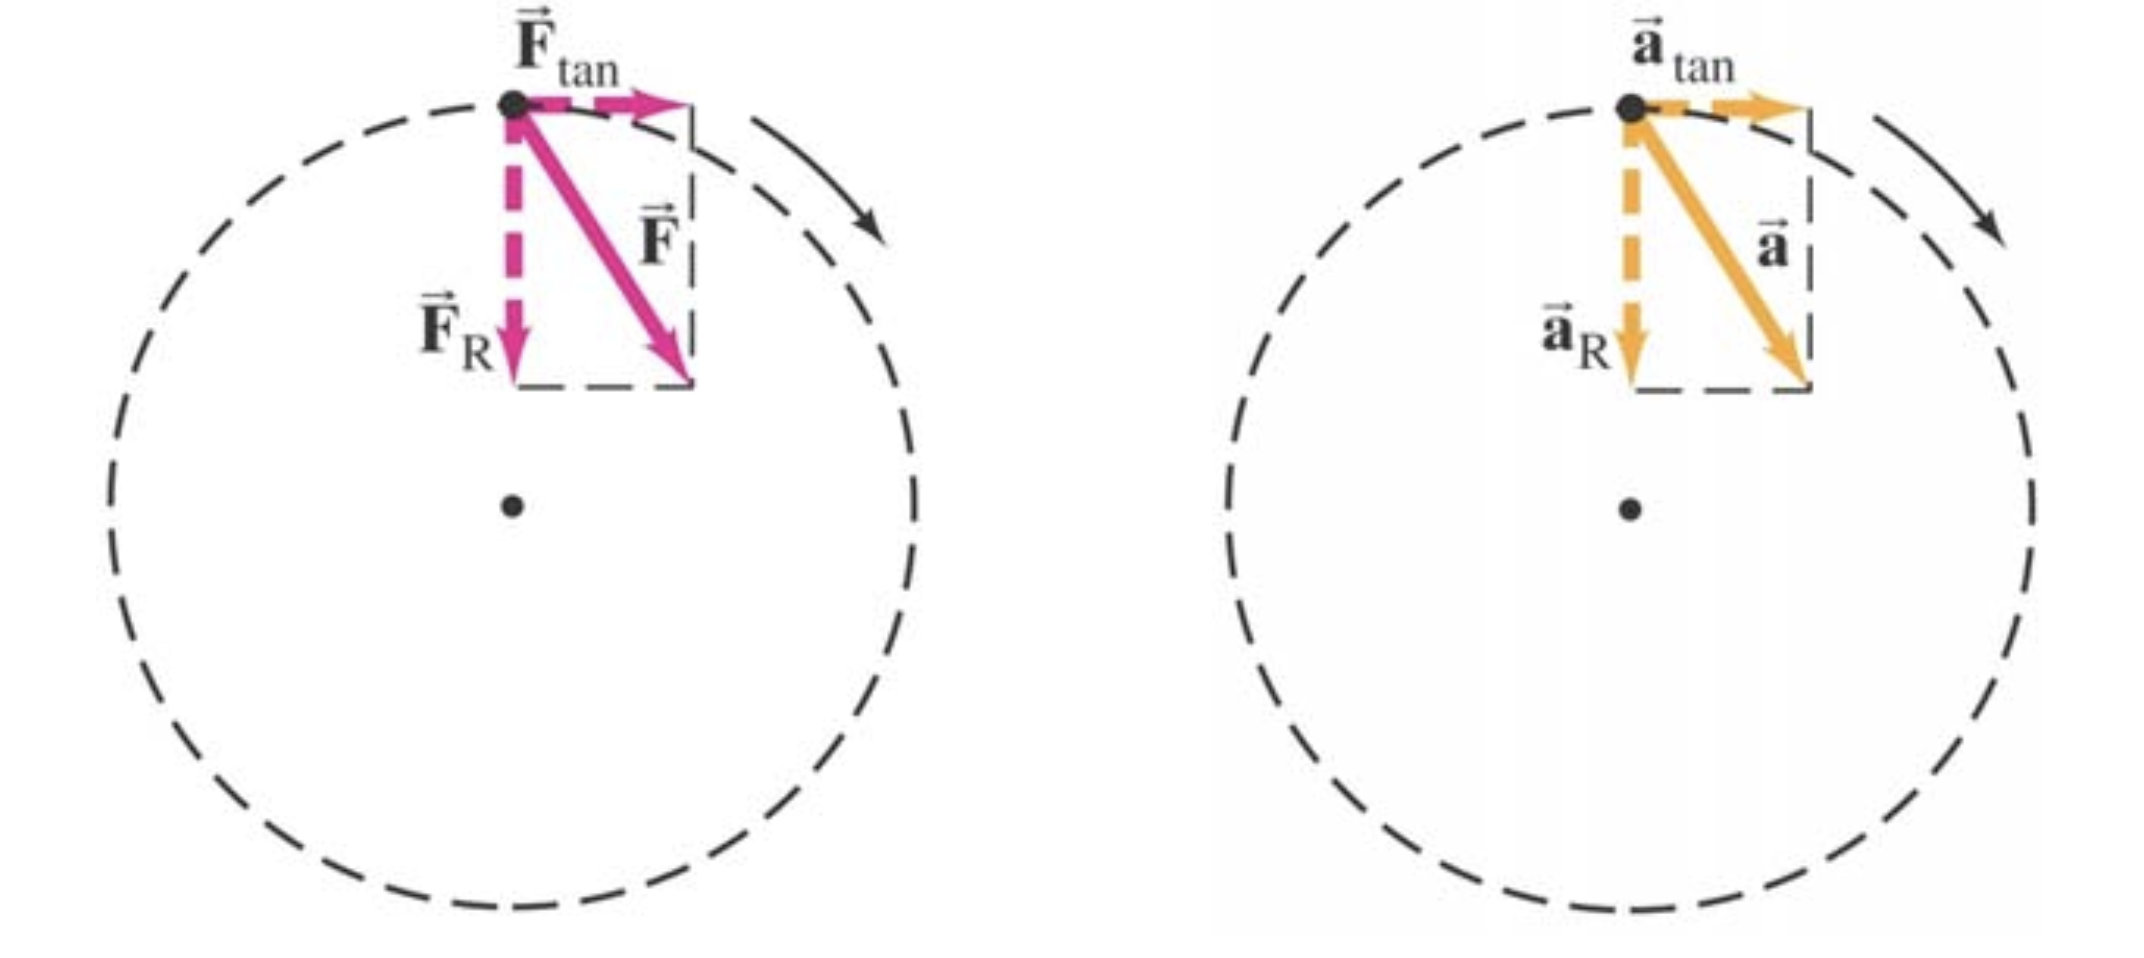
\includegraphics[scale = 0.20]{Images/Dynamica/Niet-Eenparige Cirkelbeweging.png} 
        \end{center}
\end{theo}

% \begin{ex}[Voorbeeld: Eenparige cirkelbeweging]{Eenparige cirkelbeweging}
%     \centering
%     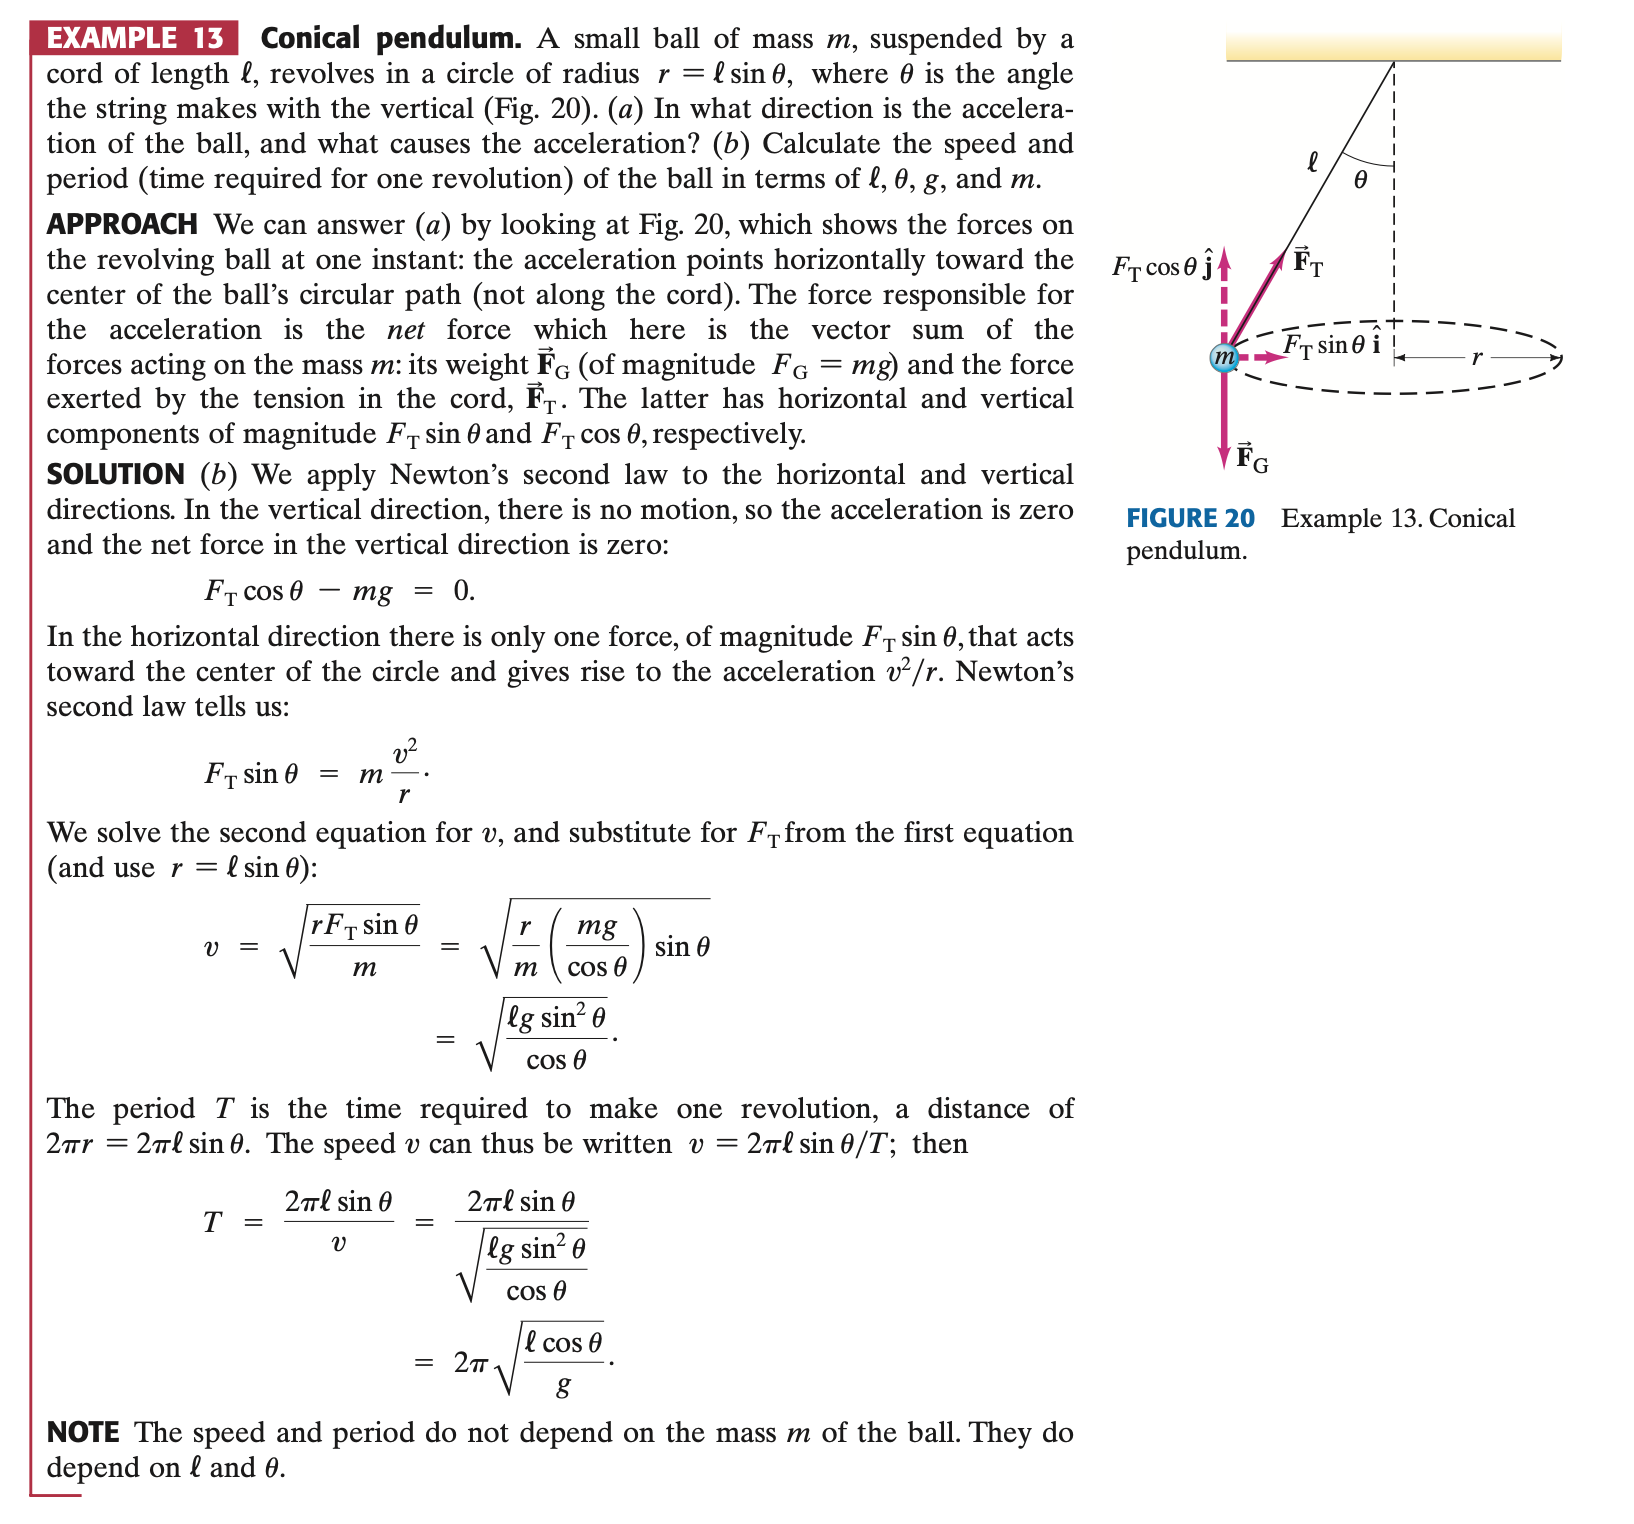
\includegraphics[scale = 0.55]{Examples/Dynamica/5.13.png}
% \end{ex}